\section{Einleitung}

\begin{figure}
\centering
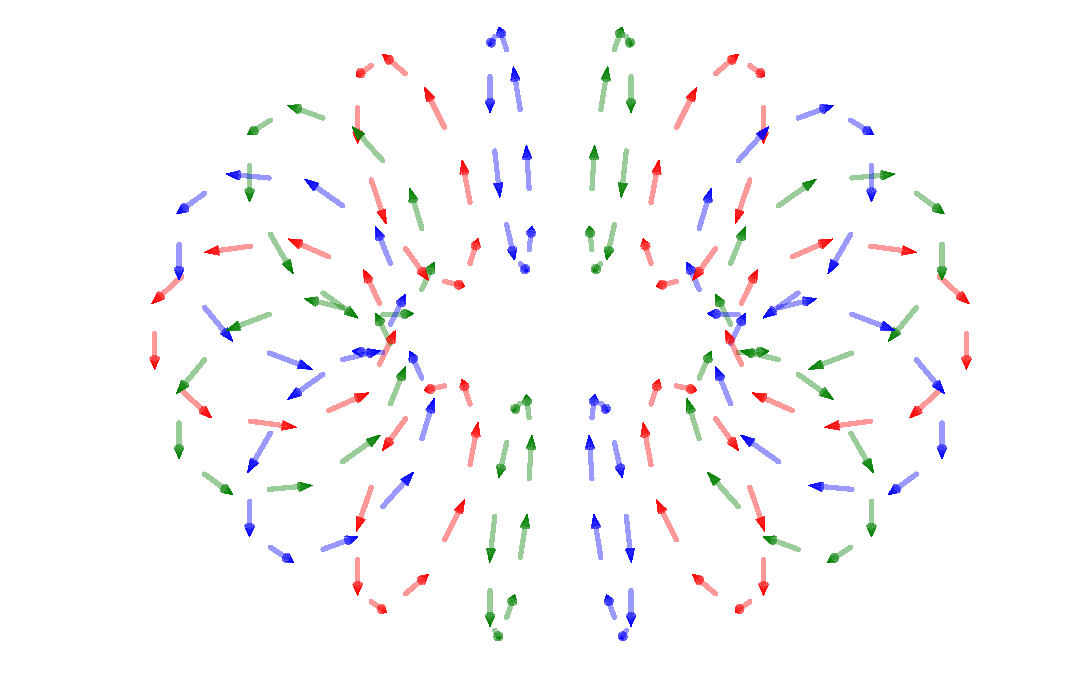
\includegraphics[width=1\textwidth]{papers/wirbelringe/fig/wirbelring_RGB.pdf}
\caption{Typischer idealer Wirbelring.
Dargestellt durch momentane Bewegungsvektoren unterschiedlicher Teilchen in regelmässigem Abstand.
Zur besseren Übersicht sind Teilchen eines Wirbels mit derselben Farbe markiert.
Unterschiedliche, benachbarte Wirbel haben unterschiedliche Farben.
Die Wirbellinie ist als schwarze, gestrichelte Linie eingezeichnet.\label{Wirbelringe:fig:generell}}
\end{figure}

\section*{Disclaimer}

In diesem Paper werden, wo nicht anders angegeben nur ideale Fluide betrachtet.

\begin{displayquote}
    The theory of inviscid fluids is the study of «dry water».

    - John von Neumann\cite{Wirbelringe:feynman1964lectures}
\end{displayquote}

\subsection{Wirbel}

Für die Betrachtung von Wirbelringen müssen wir zunächst einzelne Wirbel betrachten. 
In \ref{buch:papers:Wirbelringe:fig:flacher_wirbel} ist solch ein Wirbel abgebildet. 
\begin{figure}
\centering
\begin{tikzpicture}
\clip (-6.3,-2.7) rectangle (6.3,2.7);
\node at (-0.07,-0.07) {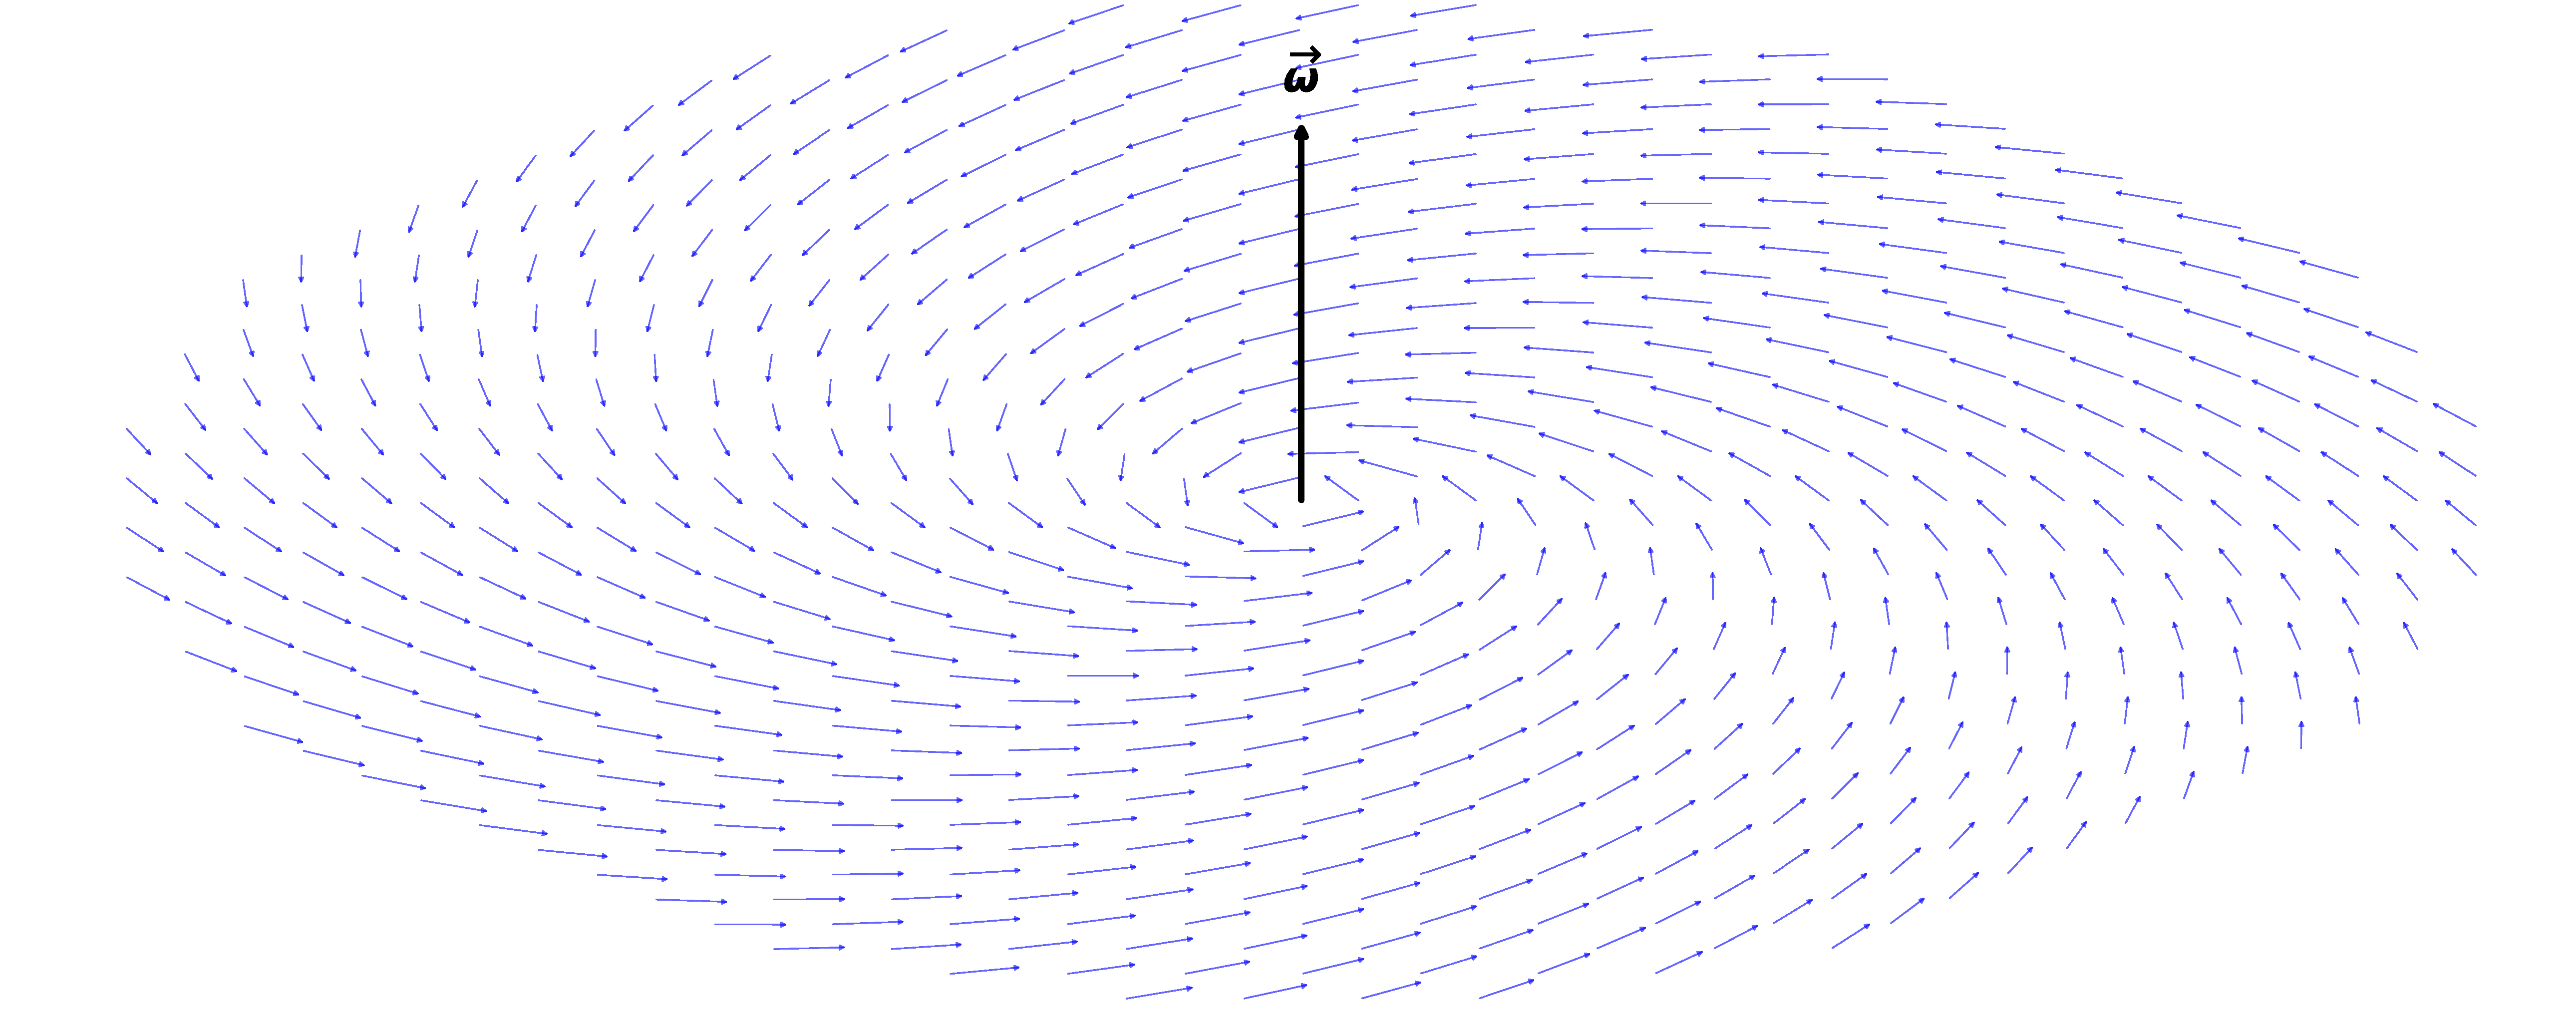
\includegraphics[width=1.08\textwidth]{papers/wirbelringe/fig/flacher_wirbel.pdf}};
%\draw[color=red] (-6.3,-2.7) rectangle (6.3,2.7);
\end{tikzpicture}
\caption{Darstellung eines 2-dimensionalen Wirbels mit Wirbelvektor
\(\vec{\omega}\).
\label{Wirbelringe:fig:flacher_wirbel}}
\end{figure}


\subsection{Wirbel vs Wirbelring}
